\section{Baseline Model}
\noindent The first and very basic model builds on the following five assumptions: (i) a single representative agent; (ii) perfect capital markets; (iii) no non-market benefits of human capital; (iv) fixed labor supply; (v) constant depreciation of human capital stock, $\sigma$. Let $T$ define a time horizon. For each $t \in T$, $H$ denotes human capital, $I \in [0,1]$ investment time, $D$ market goods that serve as inputs to the production function, and $F$ a strictly concave production function in two normal inputs. The law of motion for human capital is
\begin{equation}
\dot{H(t)} = F \left( I(t) H(t), D(t) \right) - \sigma H(t)
\end{equation}
and embeds a neutrality assumption. Namely, the current stock of human capital at time $t$, $H(t)$, and the investment time at time $t$, $I(t)$, appear as a single argument in a multiplicative fashion in the flow production of human capital. At each point of time, the current stock and the rental rate of human capital, $R$, define potential earnings
\begin{equation}
Y(t) = R H(t).
\end{equation}

\indent In general, observed earnings and potential earnings differ by two terms, foregone earnings and direct market goods costs. Let $P_{D}$ be the price of markets and define observed earnings, $E(t)$ as
\begin{equation}
E(t) = R H(t) -  R I(t) H(t) - P_{D} D(t) \label{eq:earnings}
\end{equation}
where $R I(t) H(t)$ are foregone earnings and $ P_{D} D(t) $ are direct goods costs. This expression clarifies that $I(t)$ is the fraction of time devoted to investment in each period of time. In particular, the individual occupies a fraction $I(t)$ of her human capital stock to produce a human capital flow.\\ 
\indent The individual chooses $D(t)$ and $I(t)$ to maximize her lifetime earnings stream given an initial level of human capital, $H(0) = H_{0}$. This is
\begin{equation}
\max_{D_{t}, I_{t}} \int _{0} ^{T} e^{-rt} E_{t} dt.
\end{equation}
\noindent The \textit{current value Hamiltonian} associated to the individual's problem is
\begin{equation}
\mathcal{H} (\cdot) = e^{-rt} \left[ R H(t) -  R I(t) H(t) - P_{D} D(t) \right] + \mu_{t} \dot{H(t)} 
\end{equation}
where $\mu(t)$ defines the shadow price of human capital. The first order conditions of the individual's problem are
\begin{eqnarray}
\frac{\partial \mathcal{H} (\cdot)}{\partial I(t)} = 0 &\Leftrightarrow& e^{-rt}R = \mu(t) F_{I(t)H(t)} \label{eq:focinvestment} \\
\frac{\partial \mathcal{H} (\cdot)}{\partial D(t)} = 0 &\Leftrightarrow& e^{-rt}R I(t) = \mu(t) F_{D(t)} \label{eq:focgoods} \\
\frac{\partial \mathcal{H} (\cdot)}{\partial H(t)} = - \dot{\mu(t)} &\Leftrightarrow& e^{-rt} R \left( 1 - I (t) \right) + \mu(t) \left(  F_{I(t)H(t)} - \sigma \right) = - \dot{\mu(t)} \label{eq:focstock} \\ 
\frac{\partial \mathcal{H} (\cdot)}{\partial \mu(t)} = 0 &\Leftrightarrow& \dot{H(t)} = F \left( I(t) H(t), D(t) \right) - \sigma D(t) \label{eq:focmotion} \\
\text{Transversality} &:& \lim_{t \rightarrow T} \mu(t) H(t) = 0 \label{eq:foctransversality}
\end{eqnarray}
where $F_{j} \equiv \frac{\partial F \left( I(t), D(t) \right) }{\partial j}$ for $j = D(t), I(t) H(t)$. Combine \eqref{eq:focinvestment} and \eqref{eq:focstock} to get 
\begin{equation}
\dot{\mu(t)} = - e^{-rt} R + \mu(t) \sigma \label{eq:focinvstockcombine}.
\end{equation}

\noindent Let $g(t) \equiv \mu(t) e^{rt}$ and note that $\dot{g(t)} = \dot{\mu(t)} e^{rt} + r \mu(t) e ^{rt}$. Use \eqref{eq:focinvstockcombine} to obtain 
\begin{equation}
\dot{g(t)} = (\sigma + r ) g(t) - R \label{eq:grossdep}.
\end{equation}

\indent $g(t)$ has fundamental importance to this problem because it is a discount factor that adjusts for exponential depreciation of gross investment and enables to write the individual's problem in a more intuitive way. In particular, note that \eqref{eq:foctransversality} implies that $\mu(T) = 0 $ and, therefore, $g(T) = 0$.\footnote{Note that $H(T) > 0$ because otherwise the individual losses the possibility to earn in the last period.} Thus, it is possible to solve \eqref{eq:grossdep} and obtain
\begin{equation}
g(t) = \frac{R}{\sigma + r} \left[ 1 - e^{(\sigma + r)(t - T)} \right].
\end{equation}

\indent Importantly, for an interior solution, this enables to analyze the problem in $t$ and obtain all the features of the investment dynamics and human capital accumulation. In particular, the problem of the agent is to maximize her discounted gross flow of human capital less her costs (foregone earnings plus market goods costs) 
\begin{equation}
\max_{I(t), D(t)} \left[ g(t) F(I(t) H(t), D(t)) - P_{D} D(t) - R I (t) H(t) \right]
\end{equation}
for which the first order conditions are
\begin{eqnarray}
g(t) F_{I(t)H(t)} H(t) &=& R H (t) \nonumber \\
g(t) F_{D(t)} H(t) &=& P_{D} \label{eq:newfocs}. 
\end{eqnarray}

The system in \eqref{eq:newfocs} results on a system of two equations and two unknowns that solves for the Marshallian demands of $I(t)H(t)$ and $D(t)$. Input normality together with the fact that $\dot{g(t)} < 0$ imply that the both Marshallian demands are decreasing overtime, which is intuitive because the agent faces a finite horizon problem.\footnote{Need to think why $g(t)$ is decreasing over time.} This provides the necessary arguments to analyze earnings dynamics in this first simple model.
\subsection{Earnings Dynamics}
\subsubsection{No Human Capital Depreciation}
Suppose that there is no human capital depreciation. Take the definition of earnings, \eqref{eq:earnings}, and note that
\begin{eqnarray}
\dot{E(t)} &=& R \dot{H(t)} - R \dot{I(t)H(t)} - P_{D} \dot{D(t)} \nonumber \\
           &=& R F \left( I(t) H(t), D(t) \right) - R \dot{I(t)H(t)} - P_{D} \dot{D(t)} \nonumber \\     
           &>& 0 
\end{eqnarray}

\noindent where the second equality follows from the law of motion for human capital when $\sigma = 0$.\footnote{Clear up the intuition of this result.}\\
\indent In the case of human capital depreciation earnings are not necessarily monotonic because $\dot{E(t)} = R F \left( I(t) H(t), D(t) \right) - R \sigma H(t) - R \dot{I(t)H(t)} - P_{D} \dot{D(t)}$ and $| R \sigma H(t) | $ may be big enough to make $\dot{E(t)}$ over some periods.
\subsubsection{No Depreciation and the Cobb-Douglas Production Function for Human Capital}

\noindent The simplest version of this model occurs when $\sigma = 0$ and $F(I(t) H(t), D(t))$ is a Cobb-Douglas production function. \citet{ben1967production} shows that in this case $\dot{E(t)} > 0, \ddot{E(t)} < 0$. This is, earnings increase at a decreasing rate over the life cycle.\\

\subsection{Earnings Growth Dynamics}
It is of relevance to understand how earnings behave in cases that are more general relative to Cobb-Douglas. For that sake assume that $F_{D(t)} = 0 $, i.e. assume away $D(t)$ and therefore let $F(\cdot)$ take a single argument, $I(t) H(t)$. The first order condition for investment becomes
\begin{equation}
g(t) F'(I(t) H(t)) = R
\end{equation}
and we can differentiate with respect to $t$ and get
\begin{eqnarray}
\dot{g(t)} F'(I(t) H(t)) + g(t) F''(I(t) H(t)) \dot{I(t) H(t)} &=& 0 \nonumber \\
&\Leftrightarrow& \nonumber \\
\dot{I(t) H(t)} &=& - \left( \frac{\dot{g(t)}}{g(t)} \right) \left[ \frac{F'}{F''}\right] \label{eq:itdot}.
\end{eqnarray}
\noindent Moreover, drop the argument $t$ to shorten notation, and note that
\begin{eqnarray}
\ddot{IH} = - \left[ \frac{\ddot{g}}{g} - \left( \frac{\dot{g}}{g} \right)^2 \right] \frac{F'}{F''} + \left( \frac{\dot{g}}{g} \right)^2 \left[ 1 - \frac{F'F'''}{{F''}^2} \right] \left[ \frac{F'}{F''} \right]  
\end{eqnarray}  
where we substitute in $\eqref{eq:itdot}$.\\
\indent Without lost of generality assume that $R = 1$ and note that
\begin{eqnarray}
\dot{E} &=& F(IH) - \dot{IH} - \sigma H \nonumber \\
\ddot{E} &=& F'(IH) \dot{IH} - \ddot{IH} - \sigma \dot{H} \nonumber \\
&=& \frac{1}{g} \dot{IH} - \ddot{IH} - \sigma \dot{H}.
\end{eqnarray}
Now, let $\sigma = 0$ and from \eqref{eq:grossdep} obtain $\frac{\ddot{g}}{g} = r \frac{\dot{g}}{g}$. Thus,
\begin{eqnarray}
\ddot{E} &=& - \frac{\dot{g}}{g} \frac{F'}{F''} \left[ \frac{1}{g} - \frac{\dot{g}}{g} \left( 1 - \frac{F'F'''}{{F''}^2} \right) \right] + \left[ r \frac{\dot{g}}{g} - \left( \frac{\dot{g}}{g} \right)^2 \right] \frac{F'}{F''} \nonumber \\
&=& - \frac{\dot{g}}{g} \frac{F'}{F''} \left[ \frac{1}{g} - \frac{\dot{g}}{g} \left( 1 - \frac{F'F'''}{{F''}^2} \right) - \frac{gr - \dot{g}}{g} \right] \nonumber \\
&=& - \frac{\dot{g}}{g} \frac{F'}{F''} \left[ \frac{1}{g} - \frac{\dot{g}}{g} \left( 1 - \frac{F'F'''}{{F''}^2} \right) - \frac{1}{g} \right] \nonumber \\
&=& - \left( \frac{\dot{g}}{g} \right)^2 \frac{F'}{F''} \left( 1 - \frac{F'F'''}{{F''}^2} \right)
\end{eqnarray}

\noindent where the third equality uses \eqref{eq:grossdep}, i.e. $gr - \dot{g} = 1$. F is strictly concave and therefore $-\left( \frac{\dot{g}}{g} \right)^2 \frac{F'}{F''} > 0$. The sign of $\eta \equiv \left( 1 - \frac{F'F'''}{{F''}^2} \right)$ depends on $F'''$. A sufficient condition for $\dot{E}$ to be concave is $\eta < 0$.
\begin{example} (Human Capital Production Functions and Earnings Concavity)
\begin{itemize}
\item Power Production Function 1 : consider the case of $F(x) = \frac{Ax^{\alpha}}{\alpha}$ for $ - \infty < \alpha < 1, A > 0$. Then, $\eta = \frac{1}{\alpha - 1} < 0$. Under this specification the earnings function is strictly concave with respect to time.
\item Power Production Function 2 : consider the case of $F(x) = a - b x ^ {- \alpha}$ for $ - 1 < \alpha < \infty, a,b,c > 0$. Then, $\eta = \frac{-1}{\alpha + 1} < 0$. Under this specification the earnings function is strictly concave with respect to time.
\item Quadratic Production Function: any quadratic production function has $F''' = 0$ and does not induce concavity of earnings with respect to time. 
\end{itemize}
\noindent Importantly, all this examples consider no depreciation of human capital, $\sigma = 0$. 
\end{example} 

\subsection{Specialization Period}
A period of specialization happens when the agent devotes his complete time to produce a flow of human capital, i.e. when $I(t) = 1$ for $t \in [ \underline{t}, \bar{t}]$. In order to illustrate assume away $D(t)$ so that $F_{D(t)} = 0$ and $\sigma = 0$, i.e. no human capital depreciation. First note that the marginal returns to investment decline as the stock of human capital grows and overtime. Concavity of $F(\cdot)$ causes the first implication while $\dot{g} < 0$ causes the second. Then, there is at most one period of specialization at the beginning of the time horizon, if it happens: $[0,t^*]$. This is what \citet{ben1967production} calls schooling period.\\
\indent Four conditions hold in the specialization period
\begin{eqnarray}
F'(H(t))g(t) &>& R \nonumber \\
F'(H(t^*))g(t^*) &=& R \nonumber \\
I(t^*) &=& 1 \nonumber \\
H(t^*) &=& \int \limits _{0} ^{t^*} F (H(\tau)) d\tau + H_{0} \label{eq:humantstar}
\end{eqnarray} 
\noindent where $H(t^*)$ is the human capital stock accumulated up to time $t^*$, the sum over the period $[0,t^*]$ plus the initial stock.\\
\indent Given that $R$ is fixed at $1$, any decrease in $g(t)$ lowers $t^*$ because it lowers the discount to gross investment in human capital. For example, relatively high $r$ implies relatively low $t^*$ because the individual is relatively present oriented. Also, from the \eqref{eq:humantstar}, note that a high value of $t^*$ implies lower value for $t^*$ because it takes less time to obtain $H(t^*)$.\footnote{A more realistic model, perhaps, makes $R$ depend on human capital so that more able individuals find it cheaper to invest in human capital. However, they also have higher foregone earnings and we cannot say without deeper analysis how $t^*$ behaves in such a case.} If $\sigma > 0 $ the the same conditions characterize specialization. However, the there may be more than one specialization period because, under some scenarios, a high value of $\sigma$ may knock off capital such that investment cycles are optimal. We stay away from such scenarios and keep $\sigma = 0$ in what follows.
\begin{example} (No Depreciation and the Cobb-Douglas Production Function for Human Capital: Initial Human Capital and the Specialization Period) \label{example:ndcdexample}
In this case $\dot{H} = A \left(IH \right)^\alpha$ where $0 < \alpha < 1, A>0$. As argued above, specialization happens in the period $[0,t^*]$. Thus
\begin{eqnarray}
	\alpha A \left( H(0) \right) ^{\alpha - 1 }g(0) &>& R \nonumber \\
	&\Leftrightarrow& \nonumber \\
	H(0) &<& \left[ \frac{R}{g(0)\alpha A} \right]^{\frac{1}{\alpha-1}} \label{eq:h0forspe}.
\end{eqnarray}
\indent As the conditions in \eqref{eq:humantstar} establish, the time spent in specialization is a decreasing function of $H(0)$. In this example, actually, the initial human capital needs to be below certain threshold in order for the individual to specialize during one period. 
\end{example}

\begin{example} (Infinite Horizon)
In the setting of Exercise \ref{example:ndcdexample} and if the horizon of the problem is infinite: $H(0) < \left( \frac{\alpha A}{r} \right) ^{\frac{1}{1 - \alpha}}$ because $g(t) = \frac{R}{r}$.
\end{example}

\begin{example} (No Depreciation and the Cobb-Douglas Production Function for Human Capital: the Specialization Period)
In the period of specialization $I(t) = 1$. Then,
\begin{equation}
\dot{H} = A \left( H \right)^{\alpha} \label{eq:humandiff}.
\end{equation}
The general solution for \eqref{eq:humandiff} is
\begin{equation}
H(t) = \left[ (1 - \alpha)(At + K) \right]^{\frac{1}{1-\alpha}}
\end{equation}
for some constant $K$. Given an initial condition $H(0) = H_{0}$, $K = \frac{H_{0}^{1-\alpha}}{1-\alpha}$ and
\begin{equation}
H(t) = \left[ (1 - \alpha)At + H_{0}^{1-\alpha} \right]^{\frac{1}{1-\alpha}} \label{eq:hbeforetstar}.
\end{equation}
At the end of the specialization period, as established in \eqref{eq:humantstar}:
\begin{equation}
\alpha g(t^*) A \left( H(t^*) \right)^{\alpha - 1} = R.
\end{equation}
If $T \rightarrow \infty$, $g(t) = \frac{R}{r}$ and
\begin{equation}
t^* = - \frac{H_{0}^{1 - \alpha}}{A(1 - \alpha)} + \frac{\alpha}{1 - \alpha}\frac{1}{r}. \label{eq:tstar}
\end{equation}

\indent \eqref{eq:tstar} provides some intuitive results: (i) an individual with relatively high initial human capital specializes during a relatively shorter period: $\frac{\partial t^*}{\partial       H_{0}} < 0$; (ii) a relatively abler individual specializes during relatively longer period: $\frac{\partial t^*}{\partial A} > 0$; a relatively impatient individual specializes for a relatively shorter period: $\frac{\partial t^*}{\partial r} < 0$.
\end{example}

\begin{example} (No Depreciation and the Cobb-Douglas Production for Human Capital: Post-experience Earnings)
Let $\tau = t - t^*$ define the post-school work experience and write post-school earnings as follows:
\begin{equation}
E(\tau) = R \int \limits _{0} ^{\tau} \dot{H( l + t^*)}d l + R H(t^*) - RIH(\tau + t^*).
\end{equation}
Now, from \eqref{eq:humantstar} the following equality holds:
\begin{eqnarray}
\alpha g(t) A \left( IH(t) \right)^{\alpha - 1} &=& R \nonumber \\
&\Leftrightarrow& \nonumber \\
IH(t) &=& \left[ \frac{\alpha g(t) A}{R} \right]^{\frac{1}{1-\alpha}} \label{eq:itcobb}
\end{eqnarray}
Combining \eqref{eq:itcobb} and the law of motion for human capital:
\begin{equation}
\dot{H} = A \left[ \frac{\alpha g(t) A}{R} \right]^{\frac{\alpha}{1-\alpha}} \label{eq:hdot}.
\end{equation}
Then,
\begin{equation}
E(\tau) = R \int \limits _{0} ^{\tau} A \left[ \frac{\alpha g(l + t^*) A}{R} \right]^{\frac{\alpha}{1-\alpha}} dl + RH(\tau + t^*) 
\end{equation}
and if $T \rightarrow \infty$
\begin{equation}
E(\tau) = RA \left[ \frac{\alpha A}{R} \right]^{\frac{\alpha}{1-\alpha}} \tau.
\end{equation}

\begin{center}
\begin{figure}[H]
\caption{Earnings and Experience, Cobb Douglas Technology and No Depreciation}
\centering
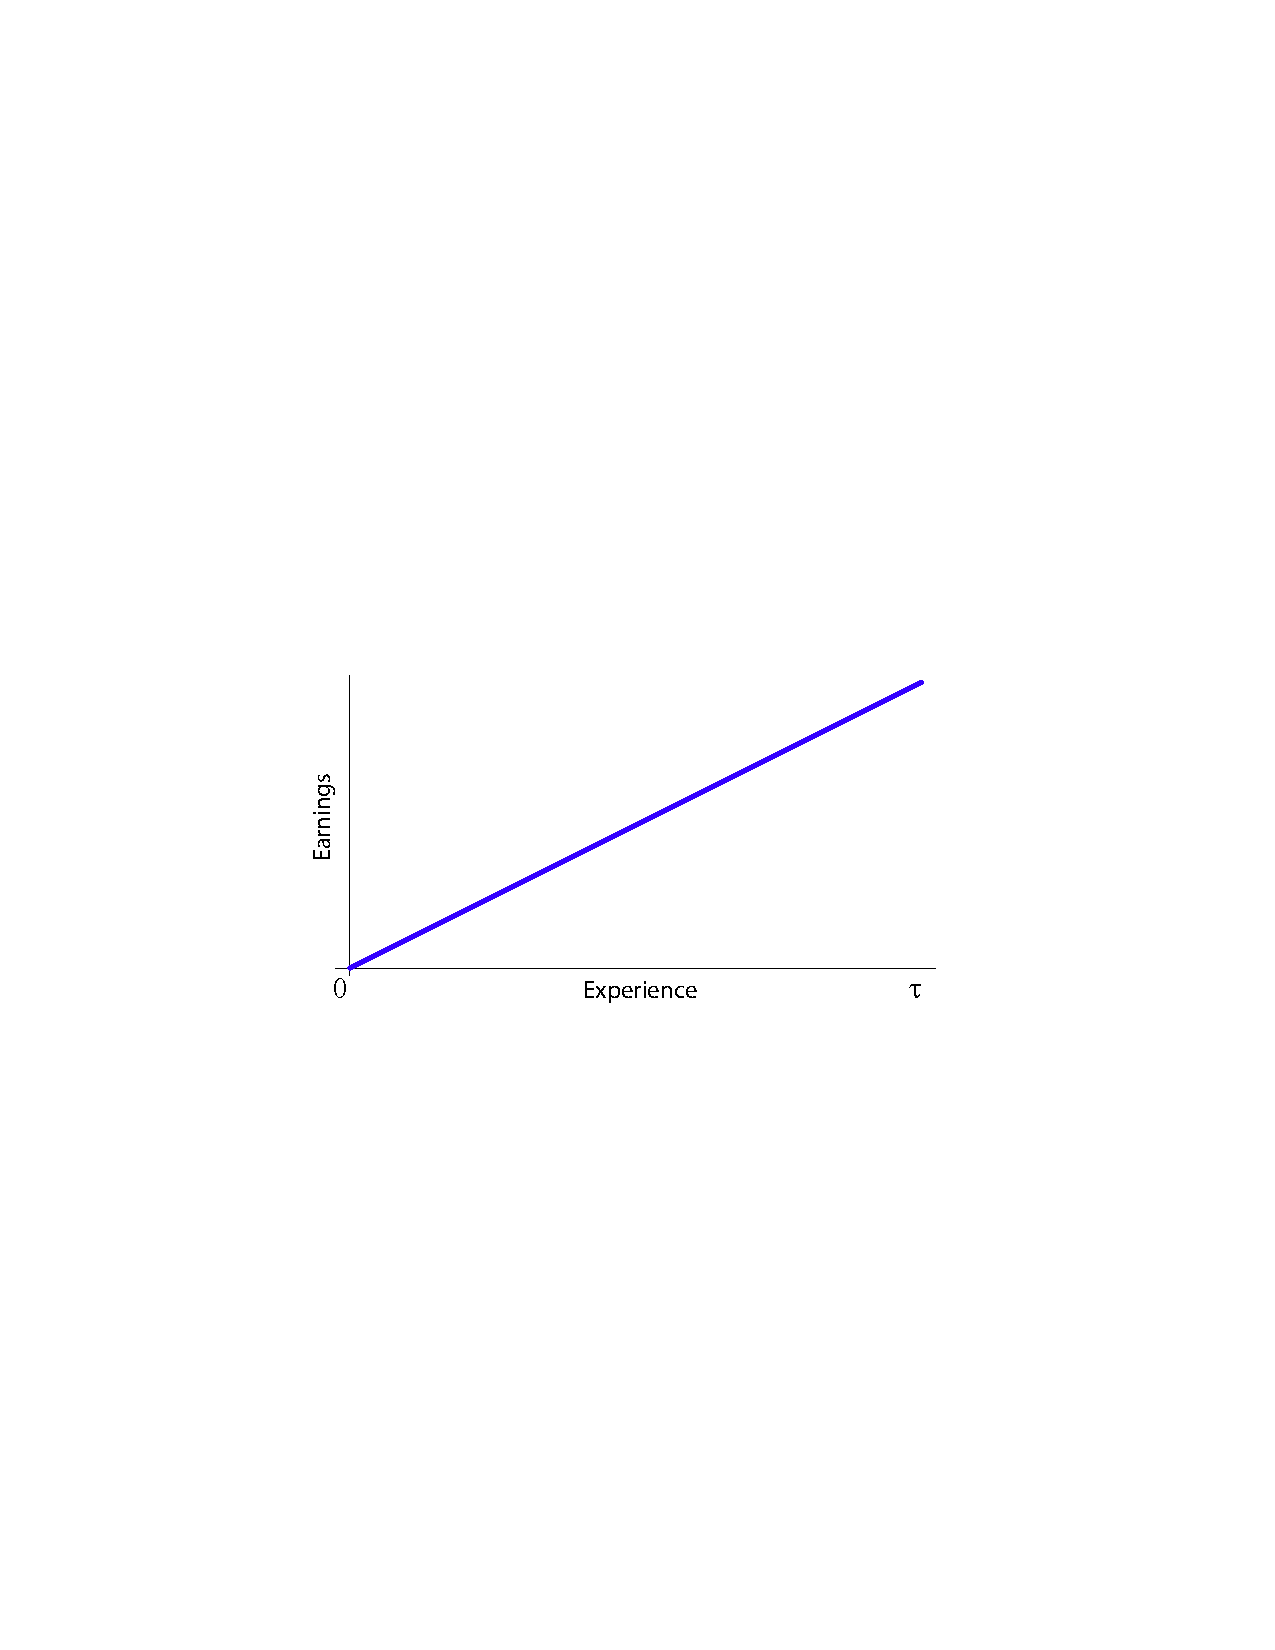
\includegraphics[width=5in, height=3in]{Figures/fig-earnings-experience.pdf}
\floatfoot{\begin{small}
Note:
\end{small}}
\end{figure}
\end{center}


\end{example}

\subsection{The Baseline Model Dynamics under the Cobb-Douglas Specification: a Summary}
This section summarizes the dynamics of the main variables in the baseline model when there is no depreciation and market goods are ruled out as inputs for the production of human capital investment. We assume that the horizon is infinite to simplify the algebra but it is important to remark that the qualitative properties of the results remain unchanged under finite horizon.

\subsubsection{Human Capital}
\begin{itemize}
\item At $t = 0$ an initial condition is given.
\item At $0 < t < t^*$ the system \eqref{eq:humantstar} provides the conditions that human capital satisfies and its expression is given by \eqref{eq:hbeforetstar}.
\item At $t = t^*$ \eqref{eq:hbeforetstar} is still a valid expression for human capital. To obtain the exact quantity it suffices to evaluate the expression for $t^*$, \eqref{eq:tstar}, into \eqref{eq:hbeforetstar}.
\item At $ t > t^* $ \eqref{eq:humantstar} and the expression for $\dot{H}$, \eqref{eq:hdot}, provide the expression for human capital.
\end{itemize}

Then,

\begin{eqnarray}
H(t) =
\begin{cases}
H_{0} & t = 0 \\
\left[ (1 - \alpha)At + H_{0}^{1-\alpha} \right]^{\frac{1}{1-\alpha}} , & 0 < t < t^* \\
\left[ \frac{\alpha A}{r} \right]^{\frac{1}{1 - \alpha}}, & t = t^* \\
\left[ \frac{\alpha A}{r} \right]^{\frac{ \alpha }{1 - \alpha}} \left( t - t^* \right) + \left[ \frac{\alpha A}{r} \right]^{\frac{1}{1 - \alpha}} , & t > t^*. \label{eq:humancapall}
\end{cases}
\end{eqnarray}

\subsubsection{Investment}
We focus on the case in which there is an specialization period, i.e. the case in which \eqref{eq:h0forspe} holds. The combination of \eqref{eq:itcobb} and \eqref{eq:humancapall} gives the following

\begin{eqnarray}
I(t) =
\begin{cases}
1, & t = 0 \\
1, & 0 < t < t^* \\
1, & t = t^* \\
\frac{\left[ \frac{\alpha A}{r} \right]^{\frac{1}{1 - \alpha}}}{\left[ \frac{\alpha A}{r} \right]^{\frac{ \alpha }{1 - \alpha}} \left( t - t^* \right) + \left[ \frac{\alpha A}{r} \right]^{\frac{1}{1 - \alpha}}}, & t > t^*. \label{eq:investall}
\end{cases}
\end{eqnarray}

\subsection{Earnings}
For the case of earnings we also on the case in which there is an specialization period, i.e. the case in which \eqref{eq:h0forspe} holds. Thus, \eqref{eq:earnings}, \eqref{eq:humancapall}, \eqref{eq:investall} define earnings as follows

\begin{eqnarray}
E(t) =
\begin{cases}
0, & t = 0 \\
0, & 0 < t < t^* \\
0, & t = t^* \\
RA \left[ \frac{\alpha A}{r} \right]^{\frac{\alpha}{1 - \alpha}} \left( t - t^* \right) , & t > t^*. \label{eq:earnsall}
\end{cases}
\end{eqnarray}







